% This is where Assessors will be looking for signs of success and for evidence of thorough and systematic 
% evaluation as discussed in Section 8.3. Sample output, tables of timings and photographs of workstation screens,
% oscilloscope traces or circuit boards may be included. A graph that does not indicate confidence intervals will 
% generally leave a professional scientist with a negative impression.

% As with code, voluminous examples of sample output are usually best left to appendices or omitted altogether.
% There are some obvious questions which this chapter will address. How many of the original goals were achieved? 
% Were they proved to have been achieved? Did the program, hardware, or theory really work?
% Assessors are well aware that large programs will very likely include some residual bugs. It should always be 
% possible to demonstrate that a program works in simple cases and it is instructive to demonstrate how close it 
% is to working in a really ambitious case.

% ~2000 words

\documentclass[final,rdr32.tex]{subfiles}
\begin{document}

\chapter{Evaluation}

This chapter describes the results obtained, as well as the evaluation methods and metrics used. Possible optimisations and relevant factors affecting accuracy are also discussed. The testing for all datasets involves few labels, due to the hardware limitations (Not enough memory to load all reference signs at the same time).

\section{LSA64 Results}

\subsection{5-label Training}

The model was tested on the LSA64 dataset, using both the basic \verb|dtw-python| implementation and the \verb|fastdtw| one. The model was trained on a sample of five different labels for sign gestures: \verb|Accept|, \verb|Appear|, \verb|Argentina|, \verb|Away|, and \verb|Barbecue|. \verb|Accept|, \verb|Appear|, and \verb|Barbecue| require both hands whereas the \verb|Argentina| and \verb|Away| can be performed with a single hand. A set of 50 videos, 10 for each label was used for testing. The accuracy for different amount of training data are as follows:

\rowcolors{2}{gray!5}{gray!30}
\begin{table}[!h]
    \begin{center}
        \begin{tabular}{ |c|c|c| }
            \hline
            Num. of videos & Accuracy (dtw-python) & Accuracy (fastdtw) \\
            \hline
            1              & 0.78                  & 0.78               \\
            5              & 0.80                  & 0.72               \\
            10             & 0.94                  & 0.74               \\
            \hline
        \end{tabular}
    \end{center}
    \caption{Results using dtw-python}
    \label{tab:accuracy}
\end{table}

As Table \ref{tab:accuracy} shows, the accuracy of the model increases as the number of training videos per label increases. \verb|dtw-python| obtains better results than \verb|fastdtw| consistently, with only the case of using a single video per label yielding a similar accuracy. This suggests that \verb|fastdtw| is as good as \verb|dtw-python| for cases where there is a low amount of training data. Further evidence is needed to make a conclusion. This will be examined in further sections.

The effect of using a different amount of training data is discussed further, including effects due to the number of hands, and how each implementation responds to different labels.

\subsubsection{Training on 1 video per label}

The overall accuracy was 78\% for both \verb|dtw-python| and \verb|fastdtw|. The distribution of correctly predicted labels is shown below:

\begin{figure}[H]
    \begin{center}
        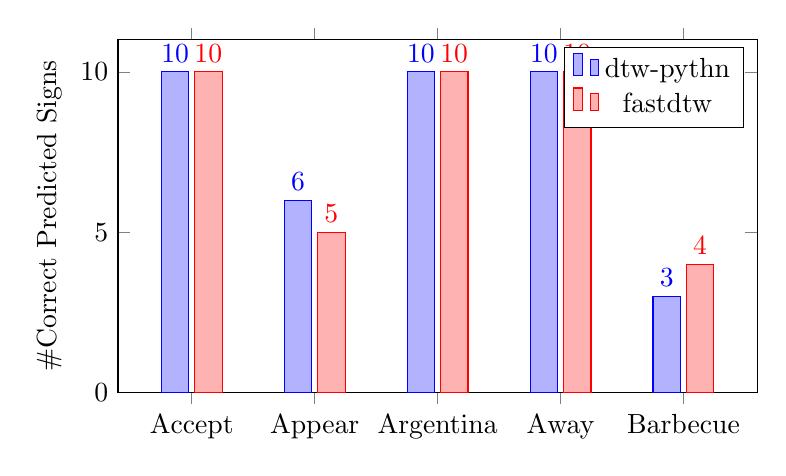
\begin{tikzpicture}
            \pgfplotsset{%
                width=.8\textwidth,
                height=.5\textwidth
            }
            \begin{axis}
                [
                    ybar,
                    enlarge x limits=0.15,
                    ymin=0,
                    ylabel={\#Correct Predicted Signs},
                    symbolic x coords={Accept, Appear, Argentina, Away, Barbecue},
                    xtick=data,
                    nodes near coords,
                    nodes near coords align={vertical},
                ]
                \addplot coordinates {(Accept,10) (Appear,6) (Argentina,10) (Away,10) (Barbecue,3)};
                \addplot coordinates {(Accept,10) (Appear,5) (Argentina,10) (Away,10) (Barbecue,4)};
                \legend{dtw-pythn, fastdtw}
            \end{axis}
        \end{tikzpicture}
    \end{center}
    \caption{\# Correctly predicted signs per label, using one video per label for training}
    \label{bar:one}
\end{figure}

\verb|Appear| and \verb|Barbecue| seem to perform poorly on both implementations. They both involve two hands, but Accept does as well and performs very well nevertheless. Other factors that might affect the accuracy could include:

\begin{itemize}
    \item \verb|Appear| is executed relatively fast, and part of the hand is hidden during the execution of the sign. This could be affecting with the mediapipe detection.
    \item \verb|Barbecue| uses both hands in a horizontal position. This seems to make it hard for mediapipe to locate the landmarks for the hands.
    \item The model might be biased in favour of \verb|Accept| due to an inherent feature of the sign gesture. This would make it seem more accurate, even if the model was predicting it for other signs.
\end{itemize}

% \newpage


\subsubsection{Training on 5 videos per label}
\label{sec:fivevid}

The \verb|dtw-python| implementation had an accuracy of 80\%, whereas the \verb|fastdtw| implementation had an accuracy of 72\%. The correct label distribution is shown below:
\begin{figure}[H]
    \begin{center}
        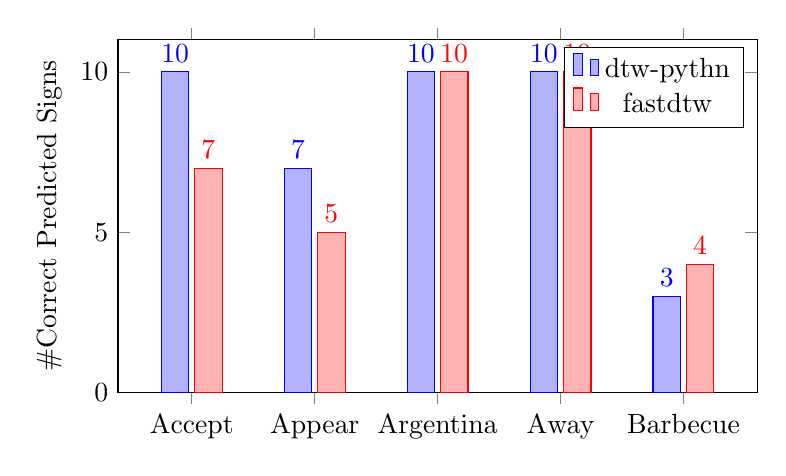
\begin{tikzpicture}
            \pgfplotsset{%
                width=.8\textwidth,
                height=.5\textwidth
            }
            \begin{axis}
                [
                    ybar,
                    enlarge x limits=0.15,
                    ymin=0,
                    ylabel={\#Correct Predicted Signs},
                    symbolic x coords={Accept, Appear, Argentina, Away, Barbecue},
                    xtick=data,
                    nodes near coords,
                    nodes near coords align={vertical},
                ]
                \addplot coordinates {(Accept,10) (Appear,7) (Argentina,10) (Away,10) (Barbecue,3)};
                \addplot coordinates {(Accept,7) (Appear,5) (Argentina,10) (Away,10) (Barbecue,4)};
                \legend{dtw-pythn, fastdtw}
            \end{axis}
        \end{tikzpicture}
    \end{center}
    \caption{\# Correctly predicted signs per label, using 5 videos per label for training}
    \label{bar:two}
\end{figure}

We note the same inconsistencies that are present in Figure \ref{bar:one}. \verb|fastdtw| also performs slightly less efficiently overall compared to \verb|dtw-python|. It is important to note however that \verb|fastdtw| gets all the signs predicted correctly for signs involving a single hand (\verb|Argentina| and \verb|Away|). This indicates possibility for optimisation in further implementations.

% \newpage

\subsubsection{Training on 10 videos per label}
\label{sec:tenvid}

The \verb|dtw-python| implementation had an accuracy of 94\%, whereas the \verb|fastdtw| implementation had an accuracy of 74\%. The correct label distribution is shown below:

\begin{figure}[H]
    \begin{center}
        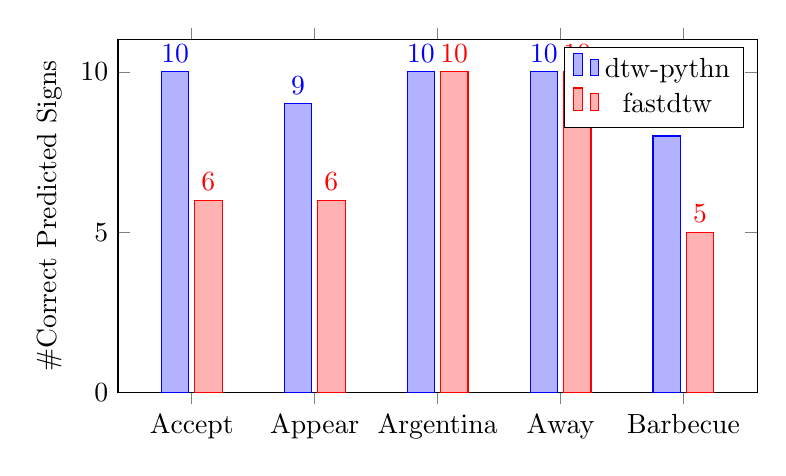
\begin{tikzpicture}
            \pgfplotsset{%
                width=.8\textwidth,
                height=.5\textwidth
            }
            \begin{axis}
                [
                    ybar,
                    enlarge x limits=0.15,
                    ymin=0,
                    ylabel={\#Correct Predicted Signs},
                    symbolic x coords={Accept, Appear, Argentina, Away, Barbecue},
                    xtick=data,
                    nodes near coords,
                    nodes near coords align={vertical},
                ]
                \addplot coordinates {(Accept,10) (Appear,9) (Argentina,10) (Away,10) (Barbecue,8)};
                \addplot coordinates {(Accept,6) (Appear,6) (Argentina,10) (Away,10) (Barbecue,5)};
                \legend{dtw-pythn, fastdtw}
            \end{axis}
        \end{tikzpicture}
    \end{center}
    \caption{\# Correctly predicted signs per label, using 10 videos per label for training}
    \label{bar:three}
\end{figure}

Accuracy is higher overall for this training set. We note the same lower accuracy for \verb|fastdtw| when it comes to two-handed signs and the same bias against \verb|Appear| and \verb|Barbecue|.

\subsection{Left-handed Videos Testing}

The model supports left-handed detection as well, even when trained on right-handed videos. Testing was conducted in a similar fashion on the same testing data used for right-handed testing, but with all of the videos flipped instead. The training data consisted of the same videos used in Section \ref{sec:fivevid}. Both the \verb|dtw-python| and \verb|fastdtw| implementations had an overall accuracy of 78\%. The distribution for correctly predicted labels is shown below:

\begin{figure}[H]
    \begin{center}
        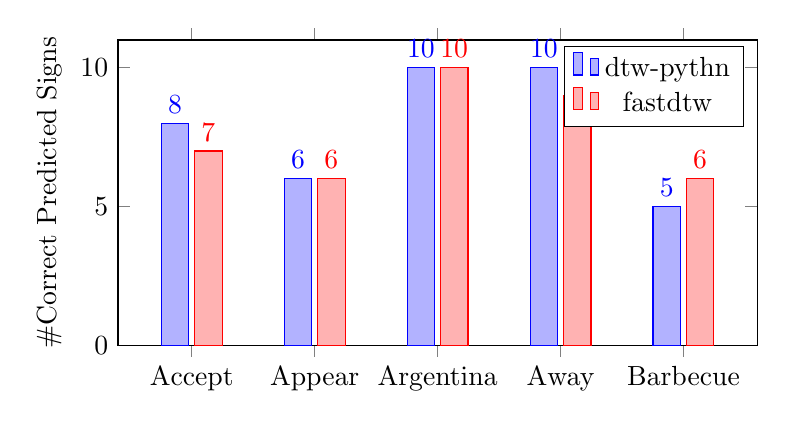
\begin{tikzpicture}
            \pgfplotsset{%
                width=.8\textwidth,
                height=.45\textwidth
            }
            \begin{axis}
                [
                    ybar,
                    enlarge x limits=0.15,
                    ymin=0,
                    ylabel={\#Correct Predicted Signs},
                    symbolic x coords={Accept, Appear, Argentina, Away, Barbecue},
                    xtick=data,
                    nodes near coords,
                    nodes near coords align={vertical},
                ]
                \addplot coordinates {(Accept,8) (Appear,6) (Argentina,10) (Away,10) (Barbecue,5)};
                \addplot coordinates {(Accept,7) (Appear,6) (Argentina,10) (Away,9) (Barbecue,6)};
                \legend{dtw-pythn, fastdtw}
            \end{axis}
        \end{tikzpicture}
    \end{center}
    \caption{\# Correctly predicted left-handed signs per label}
    \label{bar:left}
\end{figure}

We note similar results to that obtained by the model as seen in the previous sections. The overall accuracy seems to be slightly lower, despite using flipped frames for training.

\section{BSLDict Results}
\label{sec:bsldictresults}

The BSLDict dataset proved to be harder to evaluate due to its lack of suitable data. The dataset was filtered to extract labels which have a sufficient amount of data, which was $n=12$ in that case. The dataset was evaluated using both the \verb|dtw-python| and \verb|fastdtw| implementations. The labels used were \verb|Conduct|, \verb|One|, \verb|Only|, \verb|Pick|, and \verb|Stop|. \verb|One| requires a single hand to perform and the others require both hands. As many of the labels contained ambiguous data (\verb|One| contained one video for the sign representing \verb|Fourteen|, which can be inferred from the mouthing cues and comparing with existing signs), the labels were filtered again to leave the most common representations.

The testing was conducted on real-time data for this dataset. This is due to the lack of suitable data, given the size of the filtered dataset. Instead, I replicated each demonstrated sign as shown in the training videos in front of the webcam and noted the results. 20 repetitions were executed per sign as this was a reasonable amount to conduct in real-time while providing an accurate estimate of the efficiency of the model. 10 of the signs were performed right-handed and the other 10 were done left-handed. Additionally, 20 additional signs from the previous LSA64 dataset were performed in front of the model trained on the BSLDict signs to evaluate the confusion matrix. Given that the model is not optimised to detect negatives, it is expected that the model yields poor results when it comes to detecting them. However, it is of interest to know about its performance so that this aspect can be improved in future work. The model then yielded the following results on the resulting data:

\rowcolors{2}{gray!5}{gray!30}
\begin{table}[H]
    \begin{center}
        \begin{tabular}{ |c|c|c|c| }
            \hline
            Label          & Num. of training videos & Accuracy (dtw-python) & Accuracy (fastdtw) \\
            \hline
            \verb|Conduct| & 4                       & 0.80                  & 0.70               \\
            \verb|One|     & 4                       & 1.00                  & 0.95               \\
            \verb|Only|    & 4                       & 0.75                  & 0.75               \\
            \verb|Pick|    & 4                       & 0.10                  & 0.05               \\
            \verb|Stop|    & 4                       & 1.00                  & 0.95               \\
            \hline
        \end{tabular}
    \end{center}
    \caption{Results for each label}
    \label{tab:bsldictresults}
\end{table}

The model achieved an overall accuracy of 73\% using \verb|dtw-python| and 68\% using \verb|fastdtw|. The individual results are illustrated in Table \ref{tab:bsldictresults}. Additionally, the confusion matrix illustrates the number of positives and negatives for both implementations.

\rowcolors{1}{}{}
\[\begin{aligned}
        \texttt{dtw-python:}
        \begin{bmatrix}
            96 & 0 \\
            22 & 2
        \end{bmatrix}\
        \text{ }
        \texttt{fastdtw:}
        \begin{bmatrix}
            98 & 0 \\
            21 & 1
        \end{bmatrix}
    \end{aligned}\]

The results demonstrate high accuracy overall, but we also note that the sign \verb|Pick| performs poorly overall. Analysis of the training data used for it and the results leads to the following deductions:
\begin{itemize}
    \item The training data for \verb|Pick| implies that the sign for it uses only one hand, but the data itself has both hands visible, one of them resting in a neutral position. This demonstrates the need for further data pre-processing, such as cropping the frames.
    \item Many of the predictions for \verb|Pick| yielded \verb|One| instead. Both signs are relatively similar, especially compared to the other signs in the training data. This indicates that the model developed a bias for some labels, which is likely given the low amount of training data.
\end{itemize}

We also note that \verb|fastdtw| is slightly less accurate than \verb|dtw-python|, but still obtaining comparable results.

The confusion matrices shows that the model struggles to recognise negatives, mostly classifying them as signs in the training data. The lack of training data prevents the \verb|THRESHOLD| argument to be changed much in order to get more confident results.
\section{Other Studies}

The results can be compared to similar studies that have been done on the same datasets. The best performing models and their accuracies are illustrated in Table \ref{tab:studies} shown below.

\rowcolors{2}{gray!5}{gray!30}
\begin{table}[H]
    \begin{center}
        \begin{tabular}{ |c|c|c| }
            \hline
            Model                              & Dataset & Accuracy \\
            \hline
            \verb|dtw-python|                  & LSA64   & 0.94     \\
            \verb|fastdtw|                     & LSA64   & 0.78     \\
            SPOTER \cite{bohavcek2022sign}     & LSA64   & 1.00     \\
            Inception V3 \cite{rajput2022sign} & LSA64   & 0.96     \\
            \hline
        \end{tabular}
    \end{center}
    \caption{Results for each label}
    \label{tab:studies}
\end{table}

\section{User Study}

As this project involves real-time detection, a user study was conducted to measure the usability of the model in real-time and to also evaluate its accuracy on a wider range of users in real-life circumstances. The aim of the user study was to establish if the model was suitable to be used for real-time detection and if the \verb|fastdtw| implementation was faster than the \verb|dtw-python| implementation.

\subsection{Methodology}

A group of 5 participants took turns performing sign language gestures that the model is trained on. They are provided with a few examples from the testing data to familiarise themselves with the gestures. The user study is carried out separately on both the LSA64 dataset and the BSLDict dataset.

% \begin{figure}[H]
%     \begin{center}
%         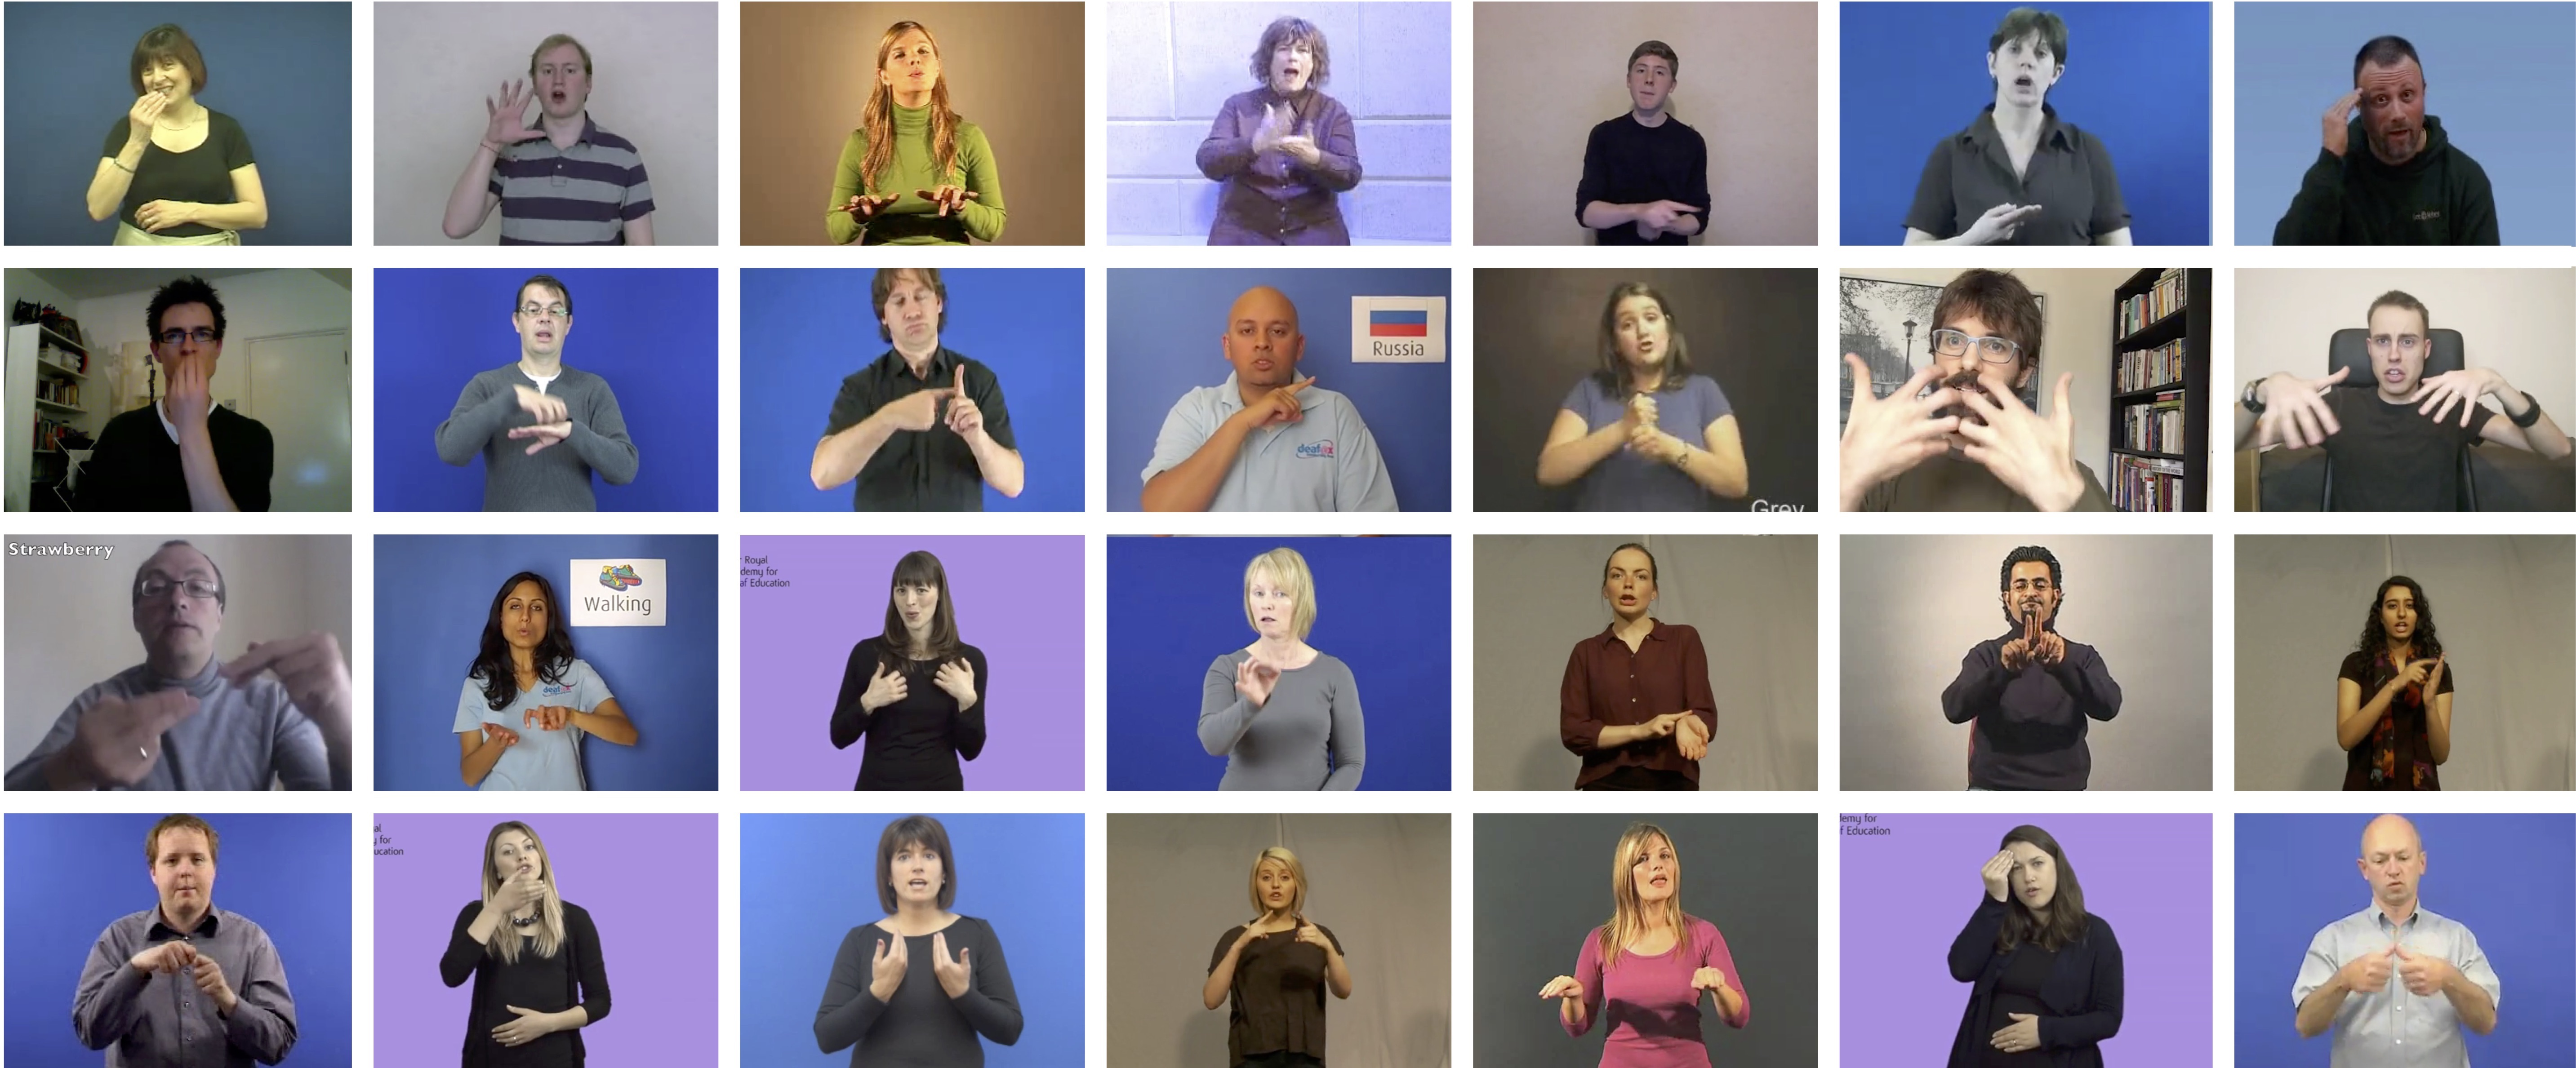
\includegraphics[scale=0.08]{images/BSLDict.jpeg}
%         \caption[caption]{User Study Examples}
%     \end{center}
% \end{figure}

\subsection{LSA64 Testing}

The model was trained on the same videos as the ones used for the \textit{10 videos per label} section in Subsection \ref{sec:tenvid}. Each user performed 10 repetitions of each sign, 5 for each implementation. This leads to a total of 50 repetitions.The results obtained are illustrated below:

\begin{figure}[H]
    \begin{center}
        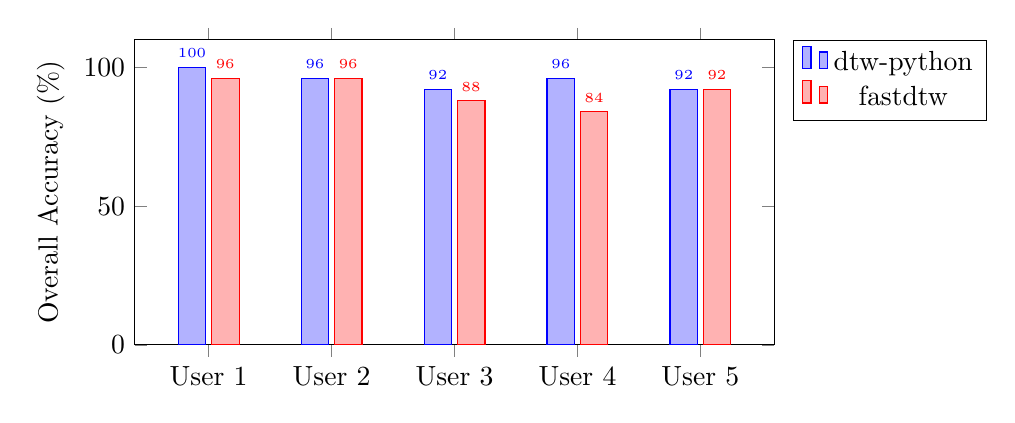
\begin{tikzpicture}
            \pgfplotsset{%
                width=.8\textwidth,
                height=.45\textwidth
            }
            \begin{axis}
                [
                    ybar,
                    enlarge x limits=0.15,
                    ymin=0,
                    ylabel={Overall Accuracy (\%)},
                    symbolic x coords={User 1, User 2, User 3, User 4, User 5},
                    xtick=data,
                    legend pos=outer north east,
                    nodes near coords,
                    nodes near coords align={vertical},
                    every node near coord/.append style={font=\tiny}
                ]
                \addplot coordinates {(User 1, 100) (User 2,96) (User 3,92) (User 4,96) (User 5,92)};
                \addplot coordinates {(User 1,96) (User 2,96) (User 3,88) (User 4,84) (User 5,92)};
                \legend{dtw-python, fastdtw}
            \end{axis}
        \end{tikzpicture}
    \end{center}
    \caption{\# Correctly predicted signs per label}
    \label{bar:lsa64user}
\end{figure}

All users obtained very high accuracy overall for both implementations. The \\ \verb|dtw-python| implementation had an overall accuracy of 95.2\% and the \verb|fastdtw| implementation had an overall accuracy of 91.2\%, for all users. The distribution of correctly predicted labels was uniform, with no sign performing noticeably better except \verb|Accept|, which was correctly predicted for all users.

\subsection{BSLDict Testing}

The model was trained on the same videos as in Section \ref{sec:bsldictresults}. The users performed 10 repetitions for each sign, 5 for each implementation. The results obtained for each user are illustrated below:

\begin{figure}[H]
    \begin{center}
        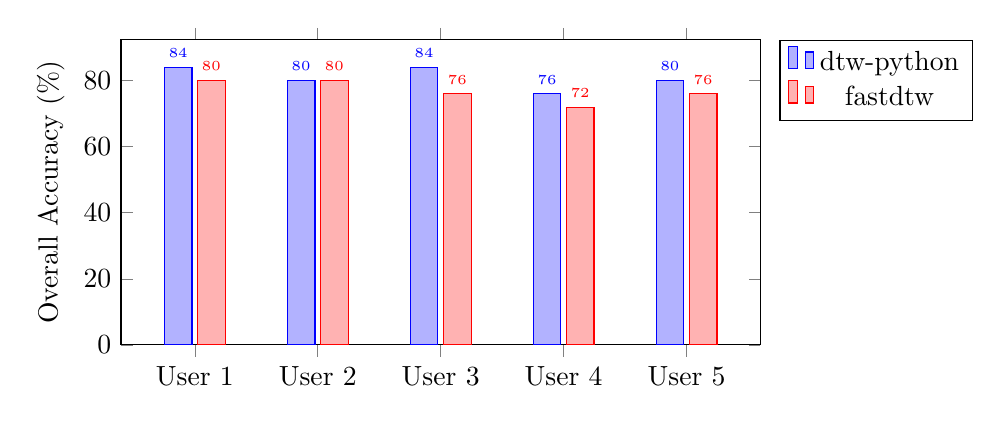
\begin{tikzpicture}
            \pgfplotsset{%
                width=.8\textwidth,
                height=.45\textwidth
            }
            \begin{axis}
                [
                    ybar,
                    enlarge x limits=0.15,
                    ymin=0,
                    ylabel={Overall Accuracy (\%)},
                    symbolic x coords={User 1, User 2, User 3, User 4, User 5},
                    xtick=data,
                    legend pos=outer north east,
                    nodes near coords,
                    nodes near coords align={vertical},
                    every node near coord/.append style={font=\tiny}
                ]
                \addplot coordinates {(User 1, 84) (User 2,80) (User 3,84) (User 4,76) (User 5,80)};
                \addplot coordinates {(User 1,80) (User 2,80) (User 3,76) (User 4,72) (User 5,76)};
                \legend{dtw-python, fastdtw}
            \end{axis}
        \end{tikzpicture}
    \end{center}
    \caption{\# Correctly predicted signs per label}
    \label{bar:bsldictuser}
\end{figure}

Users obtained less accurate results, with the \verb|dtw-python| implementation having an overall accuracy of 80.8\%, and 80.0\% for the \verb|fastdtw|. The principle reason for the low accuracy was the \verb|Pick| sign, which had an overall accuracy of 16\%, correlating with results obtained in Section \ref{sec:bsldictresults}. The reasons for this should be the same as well, and we can also exclude the possibility of the bias to be due to a specific user as well.

\subsection{User Feedback}

Users gave qualitative feedback on the evaluation process used for the user study. The overall opinion leaned towards needing to hold the signs for some period on time for signs in the LSA64 dataset, and the inaccuracy of \verb|Pick| for the BSLDict dataset. Users also did not find the need to hide the non-signing hand for single-handed signs intuitive, and would rather have both hands present on the webcam feed.

\section{Performance}
\label{sec:performance}

It is desired to test if the \verb|fastdtw| implementation provides faster computation, given that it yields less accurate predictions as seen in the previous sections. The average time used to process the extracted results from videos is used as a comparison metric. The model used the time from the evaluation of the LSA64 dataset, under the same conditions as in Section \ref{sec:fivevid}. The results are illustrated below:

\rowcolors{2}{gray!5}{gray!30}
\begin{table}[H]
    \begin{center}
        \begin{tabular}{ |c|c| }
            \hline
            Implementation    & Processing Time (s) \\
            \hline
            \verb|dtw-python| & $0.985 \pm 0.363$   \\
            \verb|fastdtw|    & $1.694 \pm 0.913$   \\
            \hline
        \end{tabular}
    \end{center}
    \caption{Average processing time for each implementation}
    \label{tab:time}
\end{table}

The results demonstrate that \verb|fastdtw| actually performs slower than the base \\ \verb|dtw-python| implementation. Given that this contradicts the previous hypothesis that \verb|fastdtw| provided an optimisation of the algorithm, further testing is done in an isolated environment. The code used to perform such testing is shown in the appendix.

Both implementations were run on randomly-generated lists with varying sizes, with the time series being compared having the same length. All computations were run a 100 times to obtain an accurate mean and standard deviation. The results are illustrated below:

\begin{table}[H]
    \begin{center}
        \begin{tabular}{ |c|c|c| }
            \hline
            Implementation    & Array Size & Processing Time (s)   \\
            \hline
            \verb|dtw-python| & 100        & $0.00084 \pm 0.00035$ \\
            \verb|dtw-python| & 1000       & $0.03945 \pm 0.00439$ \\
            \verb|dtw-python| & 10000      & $3.33221 \pm 0.06959$ \\
            \verb|fastdtw|    & 100        & $0.00415 \pm 0.00037$ \\
            \verb|fastdtw|    & 1000       & $0.05859 \pm 0.00843$ \\
            \verb|fastdtw|    & 10000      & $0.58846 \pm 0.01833$ \\
            \hline
        \end{tabular}
    \end{center}
    \caption{Average processing time for each implementation}
    \label{tab:performance}
\end{table}

\begin{figure}[H]
    \begin{center}
        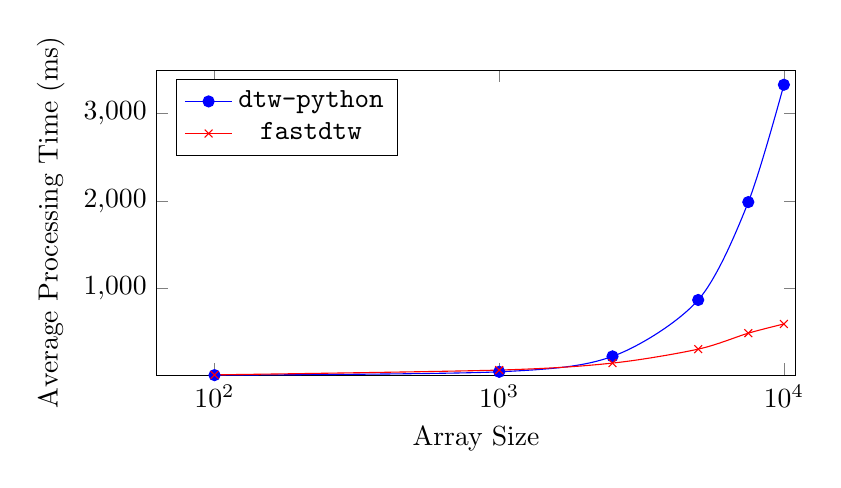
\begin{tikzpicture}
            \pgfplotsset{%
                width=.8\textwidth,
                height=.45\textwidth,
            }
            \begin{axis}[
                    xmode=log,
                    log basis x={10},
                    scaled x ticks = false,
                    xlabel=Array Size,
                    ylabel=Average Processing Time (ms),
                    xmax=11000,
                    ymin=0, ymax=3500,
                    xtick={100,1000,10000},
                    ytick={1000,2000,3000},
                    legend pos=north west,
                ]
                \addplot[smooth,mark=*,blue] plot coordinates {
                        (100,0.8)
                        (1000,39)
                        (2500,216)
                        (5000,863)
                        (7500,1986)
                        (10000,3332)
                    };
                \addlegendentry{\texttt{dtw-python}}

                \addplot[smooth,color=red,mark=x]
                plot coordinates {
                        (100,4)
                        (1000,59)
                        (2500,139)
                        (5000,299)
                        (7500,482)
                        (10000,588)
                    };
                \addlegendentry{\texttt{fastdtw}}
            \end{axis}
        \end{tikzpicture}
    \end{center}
    \caption{Variation of processing time with array size}
    \label{line:performance}
\end{figure}


The results from the isolated test shows that the processing time is dependent on the size of the array. \verb|dtw-python| grows quadratically, compared to \verb|fastdtw| which grows linearly. The difference seems to start showing when the array size is at least 2000. As such, this suggests that there is not enough data being compared to leverage the benefits of \verb|fastdtw|. A few potential ways to make full use of its performance would include:
\begin{itemize}
    \item Capturing more frames during the determined recording length. This would lead to longer lists being compared.
    \item Adapting the comparison to longer sequences, such as sign gestures that take longer to execute.
\end{itemize}

It is unclear whether the number of landmarks would affect the performance, such as including face landmarks. This is also interesting if further work is done to research the benefits of this method on continuous sign language recognition.

\end{document}